% \documentclass[a4paper, technote, compsoc]{IEEEtran}
\documentclass[../../thesis.tex]{subfiles}

\newcommand{\inner}[2]{\left<#1, #2\right>}
\newcommand{\alemap}{\ensuremath{\mathcal{A}}}
\newcommand{\dt}{\ensuremath{\Delta t}}
\newcommand{\pexp}{\ensuremath{\frac{2\gamma}{\left(\gamma-1\right)}}}
\newcommand{\aleX}{\ensuremath{\mathcal{X}}}
\newcommand{\Ah}[1]{\ensuremath{\vb{#1}^{n+1}_h}}
\newcommand{\Ahn}[1]{\ensuremath{\vb{#1}^{n}_h}}



\begin{document}

\section{One-Dimensional Gas Dynamics}
\label{sec:fom_definition}
The full order model for the parametrized one-dimensional 
piston problem is derived here.
We depart from the one-dimensional, compressible, and isentropic \mbox{Navier-Stokes} equations 
to end up with a nonlinear Burgers-like equation.
Therefore, this problem contains all the necessary ingredients to show how a ROM behaves 
in the presence of a nonlinear term within a moving domain.

The model will be derived in the continuous, semi-discrete and fully discrete contexts 
for a generic parametrization and forcing term.
We shall use the Galerkin projection principle to find a weak form, 
which we later discretize using the finite element method (FEM). 

We define the vector $\vec{\mu} \in \mathcal{P}$ to collect 
all the parameters present in the formulation.
Parameters will be present in the PDE, in the boundary conditions, 
or in the geometrical definition of the domain. 

We consider a problem with a deforming domain in time, whose movement is known and 
is thus not part of the solution:
\begin{equation*}
    \Omega(t, \vec{\mu}) := \left\{x \in \mathbb{R} : x \in \left[0, L(t, \vec{\mu})\right]\right\}.
\end{equation*}
From now on, we drop the dependency on time and the parameters unless it is strictly necessary.

\subsection{Physical Derivation}
The piston movement $L(t)$ is a real-valued smooth sinusoidal function,
\begin{equation}
    L(t) = L_0 \left[1 - \delta \left(1 - \cos \left(\omega t\right)\right)\right],
\end{equation}
where~$\omega$ is the frequency at which it oscillates, 
and \mbox{$\delta \ll L_0$} is a scale variable to adjust how much it is displaced from its original position. 
A sketch is given in Figure~\ref{fig:piston}.
The length $L_0$ is defined to keep physical dimensions sound, 
but it will be fixed to $L_0=1$ for the remainder of the work.
See Appendix~\ref{sec:appendix_piston_movement_law} 
for the derivation of this movement law.
\begin{figure}[h]
    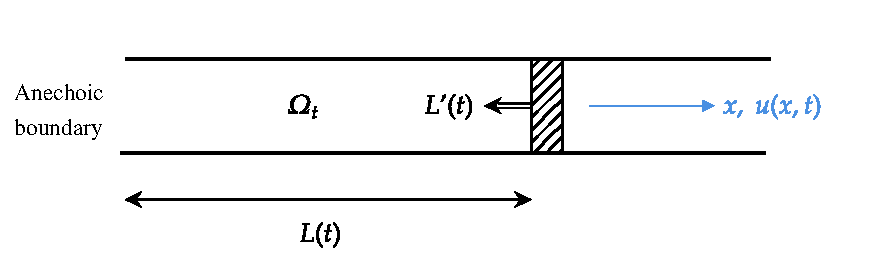
\includegraphics[width=1.05\columnwidth]{research_project/piston/figures/piston.pdf}
    \caption{Piston sketch. The flow departs from rest to the left of the piston.
    Outflow (inflow) is represented by a negative (positive) velocity value.}
    \label{fig:piston}
\end{figure}

We depart from the conservation of mass and momentum, 
and the isentropic relation between pressure and density,
\begin{subequations}
\begin{align}
    \pdv{\rho}{t} + u \pdv{\rho}{x} + \rho \pdv{u}{x} &= 0, \\ 
    \pdv{u}{t} + u \pdv{u}{x} + \frac{1}{\rho}\pdv{p}{x} &= 0, \\
    p &= k \rho^{\gamma} \label{eq:isentropic_relation}. 
\end{align}
\end{subequations}
Body forces and viscosity have been neglected for the sake of simplicity\footnote{Viscosity terms will be introduced later on for numerical stability.}.
A difficulty we find in this system for the piston application is the determination of the boundary condition for density at the piston location.
Ideally, we only want to solve an equation for the velocity, for which boundary conditions are easy to set.

To do so, we follow the steps given in \cite{nonlinearDiffusiveWaves}:
\begin{enumerate}
    \item Remove the pressure gradient through the isentropic relation. 
    \item Relate velocity~$u$ to density~$\rho$ explicitly. %with a necessary compatibility condition.
    \item Collect the results into one equation expressed in terms of the velocity~$u$.
\end{enumerate}

\subsubsection*{Pressure Gradient}
To remove the pressure gradient, we start by taking derivatives in the isentropic relation (\ref{eq:isentropic_relation}):
\begin{equation}
    \pdv{p}{x} = k \gamma \rho^{\gamma-1} \pdv{\rho}{x}
\end{equation}
Then, we recognize that the coefficients $k \gamma \rho^{\gamma-1}$ multiplying the spatial derivative of density are in fact the squared speed of sound.
From thermodynamics, the speed of sound~$a$ squared is the derivative of pressure with respect to density at constant entropy,
\begin{equation}
    a^2 = \left.\pdv{p}{\rho}\right|_S = k \gamma \rho^{\gamma-1}.
\end{equation}
Hence, the expression for the pressure gradients becomes
\begin{equation}
    \pdv{p}{x} = a^2 \pdv{\rho}{x},
\end{equation}
which can be plugged directly into the momentum equation. 
The system becomes
\begin{subequations}
\begin{align}
        \pdv{\rho}{t} + u \pdv{\rho}{x} + \rho \pdv{u}{x} &= 0, \\ 
        \pdv{u}{t} + u \pdv{u}{x} + \frac{a^2}{\rho}\pdv{\rho}{x} &= 0, \\
        a &= \sqrt{k \gamma} \rho^{\frac{\gamma-1}{2}}. 
\end{align}
\end{subequations}

\subsubsection*{Compatibility Condition between $u$ and $\rho$}
Our next step is to find a compatibility condition between the mass and momentum equations.
We define $u:=\mathtt{V}(\rho)$, which, by application of the chain rule, leads to the following equalities between the derivatives of $u$ and $\rho$ :
\begin{subequations}
    \begin{align}
        \pdv{u}{t} &= \mathtt{V}' \pdv{\rho}{t}, \\
        \pdv{u}{x} &= \mathtt{V}' \pdv{\rho}{x},
    \end{align}
\end{subequations}
where $\mathtt{V}'$ represents differentiation with respect to density.
Introducing these relations into the mass and the momentum equations to remove $u$, we obtain
\begin{subequations}
    \begin{align}
            \pdv{\rho}{t} + \pdv{\rho}{x} \left(\rho \mathtt{V}' + \mathtt{V}\right) &= 0, 
            \\ 
            \mathtt{V}' \pdv{\rho}{t} + \pdv{\rho}{x} \left(\mathtt{V} \mathtt{V}' + \frac{a^2}{\rho}\right) &= 0.
    \end{align}
\end{subequations}
Since we have an homogeneous system, it can only have a non-trivial solution if the determinant is zero.
\begin{equation}
    \begin{vmatrix}
        1 & \mathtt{V} + \rho \mathtt{V}'\\ 
        \mathtt{V}' &  \mathtt{V}\mathtt{V}' + \frac{a^2}{\rho} 
    \end{vmatrix}
    = 0
\end{equation}
This determinant implies that
\begin{equation}
    \mathtt{V}' \left(\mathtt{V} + \frac{a^2}{\rho \mathtt{V}'} - \mathtt{V} - \rho \mathtt{V}'\right) = 0.
\end{equation}
The above equation has two possible solutions, either 
\begin{equation}
    \mathtt{V}'=0 \rightarrow \mathtt{V} = C,
\end{equation} 
which is the constant solution, valid but uninteresting, or 
\begin{equation}
    \frac{a^2}{\rho \mathtt{V}'} - \rho \mathtt{V}' = 0 \rightarrow \mathtt{V}' = \pm \frac{a}{\rho}.
\end{equation}
The $\pm$ signs come up because there are two travelling waves, 
each directed to one side of the domain.
Since our piston is located at the right boundary of the domain, 
we choose the $-$ sign so that waves propagate left.
We thus imply an anechoic left boundary.
We can integrate~$\mathtt{V}'$ with respect to~$\rho$ to obtain a relation between the flow velocity~$u$ and the speed of sound~$a$:
\begin{equation}
    \mathtt{V} = - \int_{\rho_0}^{\rho} \frac{a}{\rho} d\rho 
\end{equation}
where $\rho_0$ is some reference density.
At this point it is convenient to use this reference density~$\rho_0$ to remove the constant~$k$ from the expression of the speed of sound:
\begin{subequations}
    \begin{align}
        a &= a(\rho) 
        \rightarrow 
        a_0 = a(\rho_0),
        \\
        a &= \sqrt{k \gamma} \rho^{\frac{\gamma-1}{2}} 
        \rightarrow
        a = a_0 \left(\frac{\rho}{\rho_0}\right)^{\frac{\gamma-1}{2}}.
    \end{align}    
\end{subequations}
Plugging this expression into the integral, we get
\begin{subequations}
    \begin{align}
        u = \mathtt{V} &= \frac{2a_0}{\gamma-1}\left(1 - \frac{a}{a_0}\right),
        \\[2mm]
        a &= a_0 - \frac{\gamma-1}{2}u. \label{eq:speed_of_sound_with_velocity}
    \end{align}
\end{subequations}

\subsubsection{Burgers-like Equation}
With all the above, we are now ready to obtain \textit{one} equation which contains the three departing ones.
In the momentum equation we first substitute the space derivative of density,
\begin{subequations}
    \begin{align}
        \pdv{u}{x} = \mathtt{V}' \pdv{\rho}{x} \rightarrow \pdv{\rho}{x} &= - \frac{\rho}{a} \pdv{u}{x},
        \\[2mm]
        \pdv{u}{t} + \left(u-a\right)\pdv{u}{x} &= 0.
    \end{align}    
\end{subequations}
Then, we express the speed of sound in terms of velocity (\ref{eq:speed_of_sound_with_velocity}),
which leads to a PDE containing a Burgers-like nonlinear term and 
forced convection driven by the static speed of sound, 
\begin{equation}
    \pdv{u}{t} + \frac{\gamma+1}{2}u \pdv{u}{x} - a_0\pdv{u}{x} = 0.
\end{equation}
This PDE, together with its boundary conditions and the boundary's prescribed movement, represents the mathematical model of interest for our work. 

\subsubsection{Complete Determination of Flow Variables}
Although we now have \textit{one} equation which accounts for mass conservation and the isentropic relation between pressure and density, we still have three variables. 
Computing density, pressure and the speed of sound in space and time still remains useful: 
verification of mass conservation, computation of the force exerted by the fluid at the piston, and other secondary derivations.

Since the speed of sound~$a$ is defined as a function of~$u$ in Equation (\ref{eq:speed_of_sound_with_velocity}),
once the latter is given, we can obtain density~$\rho$ and pressure~$p$ as a function of flow velocity~$u$:
\begin{subequations}
    \begin{align}
        \rho &= \rho_0 \left(\frac{a}{a_0}\right)^{\frac{2}{\gamma-1}},
        \\
        p    &= p_0 \left(\frac{\rho}{\rho_0}\right)^{\gamma},
        \\[2mm]
        \left(\frac{a}{a_0}\right) &= 1 - \frac{\gamma-1}{2}\left(\frac{u}{a_0}\right), 
        \\[2mm]
        \left(\frac{\rho}{\rho_0}\right) &= \left(1 - \frac{\gamma-1}{2}\left(\frac{u}{a_0}\right)\right)^{\frac{2}{\gamma-1}},
        \label{eq:density_as_a_function_of_speed}
        \\[2mm]
        \left(\frac{p}{p_0}\right) &= \left(1 - \frac{\gamma-1}{2}\left(\frac{u}{a_0}\right)\right)^{\frac{2\gamma}{\left(\gamma-1\right)}}.
    \end{align}
\end{subequations}

% -----------------------------------------------------------------------------
\subsubsection{Mass Conservation}
\label{sec:mass_conservation_definition}
Before we present the complete problem and its numerical solution, we comment 
on the integral equation for mass conservation.
This equation will not be explicitely used to integrate the system
(as some methods do), 
but we will use it is a numerical check 
to assess the correcteness of the results
(we expect to satisfy up to a given accuracy).

For a control volume whose boundary moves with the piston, 
the integral expression for mass conservation is
\begin{equation}
    \frac{d}{dt}\int_{\Omega_t} \rho d\Omega 
    + \int_{\partial\Omega_t} \rho \left(\vec{u} - \vec{u}_c\right) \cdot \vec{n} dS = 0
\end{equation}
At the piston location the flow moves with the piston, $\vec{u} = \vec{u}_c$, 
so the boundary integral vanishes. 
There is no flux through the walls either, so the only contribution left is the outflow.
At this location, the scalar product of the velocity and normal vectors is 
negative\footnote{Although we expect the flow to leave the domain at this point, 
which means a negative magnitude, this products needs to be done taking 
the variables positive in the direction of the axes.}, which implies
\begin{equation}
    \frac{d}{dt}\int_{0}^{L(t)} \rho(x,t) dx - \rho(0,t) u(0,t) = 0.
    \label{eq:integral_mass_conservation}
\end{equation}
If we introduce the expression for density in terms of velocity from 
Equation~(\ref{eq:density_as_a_function_of_speed}), we get
\begin{equation}
\begin{split}
        \frac{d}{dt}\int_{0}^{L(t)} \left(1 - \frac{\gamma-1}{2}\left(\frac{u(x,t)}{a_0}\right)\right)^{\frac{2}{\gamma-1}} dx 
        \\
        - u(0,t) \left(1 - \frac{\gamma-1}{2}\left(\frac{u(0,t)}{a_0}\right)\right)^{\frac{2}{\gamma-1}}  = 0,
\end{split}
\end{equation}
where the constant $\rho_0$ has cancelled out for being a common factor to both summands,
and the whole equation an equality with zero.

To ease our task at verifying this equation, we rather calculate the integral term for each time step
\begin{equation}
    I(t) = \int_{0}^{L(t)} \left(1 - \frac{\gamma-1}{2}\left(\frac{u(x,t)}{a_0}\right)\right)^{\frac{2}{\gamma-1}} dx,
\end{equation}
and only then compute time derivatives, which can be done with a second order finite difference scheme.
Then we can compute the mass defect $MD(t)$ between the time derivative of volume variation
and mass outflow at the open boundary,
\begin{equation}
    MD(t) = I'(t) - u(0,t) \left(1 - \frac{\gamma-1}{2}\left(\frac{u(0,t)}{a_0}\right)\right)^{\frac{2}{\gamma-1}}.
    \label{eq:mass_conservation_check}
\end{equation}
We shall verify to which degree of accuracy this relation is honoured by our numerical scheme.

% \mytodo{FOM: Formulate mass conservation as a FOM functional to be computed with the ROM basis.}

% \subsubsection{Interesting Physical Quantities}
% In the craft of building reduced order models, it is certainly interesting to measure and study the error between the full and reduced solutions. 
% However, in practical applications, one is often more concerned about aggregated magnitudes derived from raw flow variables, such as maximum flow, pressure gradients across channels, etc. 
% A comparison between the full order and reduced order aggregated magnitudes will shed light on the quality and reproducibility of the reduction scheme.

% We consider two magnitudes of interest:
% \begin{enumerate}
%     \item The outflow at the boundary.
%     \item The pressure gradient across the channel.
% \end{enumerate}
% The outflow at the boundary $F_L(t)$ is given by
% \begin{subequations}
%     \begin{align}
%         F_L(t) &= u(0,t) \rho(0,t),
%         \label{eq:outflow_at_the_boundary}
%         \\  
%         F_L(t) &= u(0,t) \rho_0 \left(1 - \frac{\gamma-1}{2}\left(\frac{u(x,t)}{a_0}\right)\right)^{\frac{2}{\gamma-1}}
%     \end{align}
% \end{subequations}

% The pressure gradient across the channel is the difference between pressure at the piston and at the outflow boundary,
% \begin{subequations}
%     \begin{align}
%         \Delta_L p(t) &= - \frac{p(0,t) - p(L(t),t)}{L(t)},
%         \label{eq:channel_pressure_gradient} 
%         \\ 
%         \Delta_L p(t) &= 
%         - \frac{p_0}{L(t)} 
%         \left[
%             \left(1 - \frac{\gamma-1}{2}\left(\frac{u(0,t)}{a_0}\right)\right)^{\pexp}
%         \right.
%         \\ 
%         & - 
%         \left.
%             \left(1 - \frac{\gamma-1}{2}\left(\frac{u(L,t)}{a_0}\right)\right)^{\pexp}
%         \right]
%         . \nonumber
%     \end{align}
% \end{subequations}
% We have defined it so that when the piston is moving forward, pushing the gas out of the chamber, the piston pressure gradient is defined positive.

\subsection{Continuous Formulation}
We continue with the definition of the problem in the continuous setting: 
a differential model given by a PDE and its boundary condition, referred to as {strong formulation}; 
and its weak formulation derived with the Galerkin principle.

We introduce the ALE formulation, to account for the movement of the mesh.
Then, we will introduce a scaling to work with non-dimensional variables.
This will complete the strong formulation.

Then, once we have obtained a weak formulation via the Galerkin projection principle,
we will introduce a Dirichlet lifting of the boundary conditions.
This is not a mandatory step to solve the FOM, 
since the boundary conditions can be directly set into the right-hand side of the algebraic vectors.
However, it is a paramount step for the construction of our reduced space,
to ensure the basis serves all boundary parametrizations.

\subsubsection{Strong Formulation}
At this point of the derivation, we allow ourselves to introduce an artificial viscosity term which was not present in the physical derivation of the model.
The viscosity value $\varepsilon$ will be small enough so that it does not remove 
significant amount of energy from the system, while keeping it sufficiently stable. 
More on this in Section~\ref{sec:fom_calibration_artificial_viscosity}.

Thus, the differential model in the physical space is given by the following PDE, boundary and initial conditions,
\begin{subequations}
    \begin{align}
        \left.\frac{\partial u}{\partial t}\right|_{x} 
        + \frac{\partial u}{\partial x}\left(\frac{\gamma+1}{2}u - a_0\right) 
        - \varepsilon \pdv[2]{u}{x} &= 0, \label{eq:1d_fom_strong_pde} \\
        % \frac{\partial u}{\partial x}(0, t) &= 0, \\
        u(L, t) &= L'(t),
        \\
        \lim_{x\rightarrow-\infty}u(x,t) &= 0,
        \label{eq:rest_condition_at_infinity}
        \\
        u(x, 0) &= 0. 
    \end{align}
\end{subequations}
The notation for the time derivative,
\begin{equation*}
    \left.\frac{\partial u}{\partial t}\right|_{x},
\end{equation*}
indicates that the derivative takes place in the physical domain. 
This is relevant for the ALE formulation, which we explain in the following section.

\subsubsection{Boundary conditions}
At the right boundary (moving piston) a Dirichlet condition sets the flow velocity equal to the one of the moving wall,
\begin{equation}
    L'(t) = - \delta L_0 \omega \sin(\omega t).
\end{equation}
At the left boundary, we have to find a procedure to model 
the condition that our piston tube is infinite, 
and hence that the far region of the flow is not aware of the piston's motion. 
This is an artificial boundary condition, which we choose to deal with by
setting the normal derivate in space to zero
\begin{equation}
    \pdv{u}{x} \qty(0, t) &= 0.
\end{equation}
This simplified model reflects that, due to the absence of
incoming waves from the infinite tube,
the solution does not change in space once it is far away from the piston motion.
% We postpone this discussion for the moment,
% since the PDE needs to be further modified to account for the 
% moving mesh in the physical domain.
% We shall deal with it once we are dealing with the weak form,
% in Section~\ref{sec:outer_boundary}.

\subsubsection{ALE Formulation}
Despite the fact that we will be solving the problem in the physical moving domain, 
we still need the two basic ingredients stemming at the root of the ALE method:
\begin{itemize}
    \item a smooth mapping between domains;
    \item a mesh velocity vector.
\end{itemize}

We introduce the ALE mapping 
\mbox{$\alemap : \Omega_0 \rightarrow \Omega_t$ }
that connects a point in the fixed reference domain $\mathcal{X}$ with a point in the physical domain $x$,
\begin{subequations}
    \begin{align}
        x &= \alemap(\aleX, t), \\
        \aleX &= \alemap^{-1}(x, t).
    \end{align}
\end{subequations}
We assume this map to be regular enough for all the operations that we will carry with it.
Then, we define the mesh velocity $w_m(x,t)$ function as the time derivative of the spatial coordinate, which will coincide with the time derivative of the ALE map:
\begin{equation}
    w_m(x,t) = \pdv{x}{t} = \pdv{\alemap}{t} \ (x, t) = \pdv{\alemap}{t} \ (\alemap(\aleX,t), t).
\end{equation}
% Due to our algebraic approach, this mesh velocity can be computed in the 
% reference domain $\aleX$.
% This will produce the same vector values as if we actually computed and evaluated
% the inverse mappin since i

\subsubsection{ALE: Uniform Stretching}
\label{sec:ale_uniform_stretching}
For the moving piston, a simple mapping can be derived, 
rescaling the spatial variable with the piston length in time,
\begin{equation}
    \aleX = \frac{x}{L(t)} \rightarrow \alemap(\aleX, t) = \aleX L(t), \, \aleX \in [0,1].
\end{equation}
Then, we have an analytical expression for the mesh velocity too,
\begin{equation}
    w_m(x,t) = \pdv{\alemap}{t} = \aleX L'(t) = L'(t) \qty(\frac{x}{L(t)}).
\end{equation}
The mesh velocity results in a linear interpolation 
of the moving boundary velocity.

Additionally, we introduce the Jacobian of the ALE mapping. 
The Jacobian is defined as the determinant of the ALE mapping gradient,
\begin{equation}
    J_{\alemap} = \qty|\pdv{x}{\aleX}|.
    \label{eq:Jacobian}
\end{equation}
The Jacobian is used when we want to map an integral in the physical domain
into an integral in the reference, fixed domain,
\begin{equation}
    \int_{\Omega_t} \phi \dd \Omega = \int_{\Omega_0} \phi J_{\alemap} \dd \Omega.
    \label{eq:jacobian_integral_transformation}
\end{equation}
% Equation~\eqref{eq:jacobian_integral_transformation} 
% gives us information about the difficulty we face reducing the algebraic operators.
% Although we will not be using this transformation explicitly in our calculations,
% it is useful to see it written down to understand any possible nonlinearities
% that arise from the ALE formulation.
For our piston-like one-dimensional geometry, we have a very simple transformation,
\begin{equation}
    J_{\alemap} = L(t),
    \label{eq:jacobian_trivial}
\end{equation}
which spreads out the deformation of the domain uniformly across all the mesh elements.
Since the Jacobian does not depend on space,
we could pull it out of the integral, 
\begin{equation}
    \int_{\Omega_t} \phi \dd \Omega 
    = 
    \int_{\Omega_0} \phi L(t) \dd \Omega
    =
    L(t) \int_{\Omega_0} \phi \dd \Omega.
    \label{eq:jacobian_pulled_out_integral}
\end{equation}
That is, the Jacobian transformation for a piston-like motion 
does not introduce any nonlinearity in the space dimension. 
We will come back to this fact further down in the document,
when we comment upon the reduction of the algebraic operators.

At last, we can carry out a \textit{correctness} check in our calculations 
by attempting to verify a well known relation between 
the mesh velocity vector and the Jacobian \cite{aris1990vectors},
\begin{subequations}
    \begin{align}
        \pdv{J_{\alemap}}{t} &= J_{\alemap} \nabla \cdot w_m,
        \label{eq:jacobian_derivative}
        \\[2mm]
        \pdv{J_{\alemap}}{t} &= L'(t),
        \\
        J_{\alemap} \nabla \cdot w_m 
        &= L(t) \frac{L'(t)}{L(t)} 
        = L'(t),
    \end{align}
\end{subequations}
which proves the identity.
Equation~\eqref{eq:jacobian_derivative} could be part of our problem 
if we did not have access to an explicit expression for the Jacobian, 
and we wanted to solve our problem in a fixed reference domain. 
It is an ODE whose initial condition would be 
$J_{\alemap}(0) = 1$
if the reference domain coincided with the initial domain configuration of the transient domain.

\subsubsection{ALE: Non-Uniform Mesh Displacement}
We also introduce a non-uniform distortion to the nodes,
to mimick the effects of mesh adapting techniques.
As a proxy, we take a generic density function with a Gaussian bell,
\begin{equation}
    \mathcal{F}\qty(\aleX) &= y_c \cdot \exp(-\qty(\frac{\aleX - x_c}{\sigma_c})^2),
\end{equation}
where three geometrical parameters are defined:
\begin{itemize}
    \item $x_c$: location;
    \item $\sigma_c$: span,
    \item $y_0$: magnitude.
\end{itemize}
This will concentrate nodes on a specific region of the domain.
Then, for $\aleX \in \Omega_0$, where $\Omega_0 = \qty[0, L_0]$ is the fixed reference domain,
we have the following transformation in terms of a mesh displacement,
\begin{subequations}
    \begin{align}
        x &= \aleX + d\qty(\aleX, t),
        \label{eq:displacement_definition}
        \\[2mm]
        d\qty(\aleX, t) &= \aleX \cdot \qty[1 + \mathcal{F}\qty(\aleX)] \qty(\hat{L}(t) - 1),
        \\[2mm]
        \hat{L}(t) &= 1 - \delta \cdot \qty(1 - \cos(\omega t)).
    \end{align}
\end{subequations}
This displacement contains the piston oscillation 
and the non-uniform concentration of the nodes.

\subsubsection*{Effects on the Mesh Size}
We demonstrate the effects of the non-uniform displacement in the mesh step size.
By evaluating Equation~(\ref{eq:displacement_definition}) at two consecutive nodes
and computing their difference,
\begin{subequations}    
\begin{align}
    \Delta x_i &= x_i - x_{i-1},
    \\[2mm]
    \Delta x_i &= \aleX_i - \aleX_{i-1} + \qty(d\qty(\aleX_i, t) - d\qty(\aleX_{i-1}, t)),
    \\[2mm]
    \Delta x_i &= \Delta \aleX_i + \qty(d\qty(\aleX_i, t) - d\qty(\aleX_{i-1}, t)),
    \\[2mm]
    \Delta x_i &= 
    \underbrace{\Delta \aleX_i \cdot \hat{L}(t)}_{\text{Uniform stretching}}
    \nonumber\\
    &+\qty[\aleX_i \cdot \mathcal{F}\qty(\aleX_i)
    - \aleX_{i-1} \cdot \mathcal{F}\qty(\aleX_{i-1})] \cdot \qty(\hat{L}(t) - 1);
    \end{align}
\end{subequations}
we arrive to an expression for the mesh size $\Delta x_i$ 
as a function of the reference mesh size and nodes position.
If the function $\mathcal{F}$ was set to zero, 
we recover the uniform stretching derived in Section~\ref{sec:ale_uniform_stretching}.

\subsubsection{Time Derivative in the Reference Domain}
Since the equations are to be solved in the physical domain, 
we need to adjust the time derivative in the physical domain 
$\left(\left.\frac{\partial u}{\partial t}\right|_{x}\right)$, 
so that it takes into account the movement of the mesh nodes.
By application of the chain rule we get
\begin{equation}
    \left.\frac{\partial u}{\partial t}\right|_{\aleX} = 
    \left.\frac{\partial u}{\partial t}\right|_{x} + w_m \pdv{u}{x},
\end{equation}
from where we get the necessary modification to the strong form (\ref{eq:1d_fom_strong_pde}) of the PDE, 
\begin{equation}
    \left.\frac{\partial u}{\partial t}\right|_{\aleX} 
    + \left(\frac{\gamma+1}{2}\right) u \frac{\partial u}{\partial x} 
    - \left(a_0 + w_m\right)\frac{\partial u}{\partial x} 
    - \varepsilon \pdv[2]{u}{x} = 0.
\end{equation}
An additional convective term shows up, to take into account the movement of the nodes.
We will show in the results section how, if we remove this term, mass is no longer conserved.

% -----------------------------------------------------------------------------
\subsubsection{Dimensionless Equations}
Finally, we carry out a non-dimensionalization of the velocity and the spatial coordinate,
\begin{subequations}
    \begin{align}
        \tilde{x} = \frac{x}{L_0}, \qquad \tilde{u} = \frac{u}{a_0},
    \end{align}
\end{subequations}
with respect to the static speed of sound~$a_0$ and the piston's initial length~$L_0$.
This leads to the PDE and boundary condition
\begin{subequations}
    \begin{align}
        \pdv{\tilde{u}}{t} 
        + \left(\frac{\gamma+1}{2}\right)\left(\frac{a_0}{L_0}\right) \tilde{u} \pdv{\tilde{u}}{\tilde{x}}
        - \left(\frac{\varepsilon}{L_0^2}\right) \pdv[2]{\tilde{u}}{\tilde{x}}
        \nonumber
        \\[2mm]
        - \left(\frac{a_0}{L_0}\right)\left(1 + \frac{w_m}{a_0}\right)\pdv{\tilde{u}}{\tilde{x}}
         &= 0, 
        \\[2mm]
        \tilde{u}(L(t),t) = \frac{L'(t)}{a_0} &= b_L(t).
    \end{align}    
\end{subequations}
For the sake of clear notation, we condense the coefficients 
% which multiply the function and its derivatives,
\begin{subequations}
    \begin{align}
        b_0    &= \frac{a_0}{L_0} \left(\frac{\gamma+1}{2}\right), 
        \\[2mm]
        b_L(t) &= - \frac{\delta L_0 \omega}{a_0} \sin(\omega t),
        \\[2mm]
        c(x,t) &= \left(\frac{a_0}{L_0}\right)\left(1 - \frac{w_m}{a_0}\right),
    \end{align}
\end{subequations}
and drop the $\tilde{u}$ notation to avoid an overloaded notation.
The coefficient 
\begin{equation}
    u_p = \left(\frac{\delta L_0 \omega}{a_0}\right)    
\end{equation}
multiplying the boundary condition
is the ratio between the piston motion and the static speed of sound\footnote{
    A proxy for the average speed at which information propagates.
    }.
It is the maximum piston mach number, in terms of the static speed of sound.
This coefficient will drive the response of the fluid 
to the motion of the piston.
The larger it is, 
the stronger the nonlinear response will become (steepening shock wave). 
% We shall exploit this fact to build our reduced space, by sampling smartly through the parameter space.

With all of this done, we obtain a familiar PDE structure with diffusion, 
linear and nonlinear convection terms:
\begin{equation}
    \left.\frac{\partial u}{\partial t}\right|_{\aleX} 
    + b_0 u \frac{\partial u}{\partial x} 
    - c(x,t)\frac{\partial u}{\partial x} 
    - \varepsilon  \pdv[2]{u}{x} = 0.
\end{equation}
% Before moving on to the derivation of the weak formulation, we apply the scaling to the mass conservation.

\subsubsection{Dimensionless Mass Conservation}
If the former rescaling is applied, Equation~(\ref{eq:mass_conservation_check}) 
for mass conservation needs to be updated, 
to take into account the fact that the velocity variable is now scaled with the speed of sound.
\begin{subequations}
    \begin{align}
        I(t) &= \int_{0}^{\frac{L(t)}{L_0}} 
        \left(1 - \frac{\gamma-1}{2}u(x,t)\right)^{\frac{2}{\gamma-1}} 
        \dd x, 
        \\
        \frac{MD(t)}{\rho_0 a_0} &= \frac{1}{a_0}I'(t) - u(0,t) 
        \left(1 - \frac{\gamma-1}{2}u(0,t)\right)^{\frac{2}{\gamma-1}}.
    \end{align}    
\end{subequations}

% \subsubsection{Derived Variables}
% The derived magnitudes of interest, Equations~(\ref{eq:channel_pressure_gradient}) and~(\ref{eq:outflow_at_the_boundary}), have to be rescaled too:
% The outflow at the boundary $F_L(t)$ is given by
% \begin{equation}
%     F_L(t) = a_0 \rho_0 u(0,t) \rho(0,t).
% \end{equation}

% The pressure gradient across the channel is the difference between pressure at the piston and at the outflow boundary,
% \begin{equation}
%     \Delta_L p(t) = - \frac{p(0,t) - p(L(t),t)}{L(t)}. 
% \end{equation}
% We have defined it so that when the piston is moving forward, pushing the gas out of the chamber, the piston pressure gradient is defined positive.
% % \subsubsection*{Geometric Conservation Laws}

\subsubsection{Weak Formulation}
Since we will be working with the Galerkin procedure to solve PDEs, 
we define the $L^2(\Omega)$ inner product to transform the strong formulation into a weak, variational one,
\begin{equation}
    %\inner{u}{v}_{(t, \mu)} = \int_{\Omega(t, \mu)} uv\ d\Omega.
    \inner{u}{v} = \int_0^L uv\ \dd\Omega.
\end{equation}
This inner product induces the so called \emph{eyeball} norm, 
if two functions \textit{look} alike $\norm{f-g}$ will return a small value,
\begin{equation}
    % \norm{f-g}_{(t, \mu)}  = \sqrt{\int_{\Omega(t, \mu)} (f - g)^2\ d\Omega}.
    \norm{f-g}  = \sqrt{\int_0^L (f - g)^2\ \dd\Omega}.
\end{equation}
% Eventually, we will also be interested in other norms, such as the $H^1(\Omega)$ norm, which captures the differences in the gradients too.
% This is important when computing stress-related values from the solved field.
With this inner product, we project the residual of the strong formulation onto a given fuction 
$u, v \in V$,
where $V$ is a suitable Hilbert space,
\begin{subequations}
    \begin{align}
        \label{eq:1d_fom_weak_formulation}
        \inner{\frac{\partial u}{\partial t}}{v} 
        \textcolor{NavyBlue}{+ \inner{b_0 u \grad u}{v}}
        \textcolor{Purple}{- \inner{c \grad u}{v}} 
        \nonumber \\ 
        \textcolor{OliveGreen}{+ \inner{\varepsilon \grad u}{\grad v}} 
        + \textcolor{OliveGreen}{\varepsilon \left.\pdv{u}{x}\right|_{x=0} v}
        &= 0,  
        \\[2mm]
        u(x, 0) &= 0, 
        \\
        \pdv{u}{x} \qty(0, t) &= 0,
        \\
        u(L, t) &= b_L(t);
        \\[2mm]
        b_L(t) &= - \frac{\delta L_0 \omega}{a_0} \sin \omega t.
    \end{align}
\end{subequations}
% The outflow Neumann condition has been taken into account, but since it is homogeneously zero, it does not show up. 
% The natural boundary condition, which for this problems translates into an homogeneous Neumann condition,
%has already been taken into account in the integration by parts procedure of the diffusion term. 

% \subsubsection{Natural Outer Boundary Condition}
% \label{sec:outer_boundary}
% In this section we explore how to deal with the rest condition at infinity, 
% Equation~\eqref{eq:rest_condition_at_infinity}. 
% We follow the reasonings found in \cite{outerBoundary},
% which are validated later on by the convergence of consistency checks
% such as the mass conservation equation, see Section~\ref{sec:fom_calibration_bdf_convergence_rates}.

% Since we have a finite domain, which goes from the origin to the piston location,
% we need to determine a boundary condition which allows us 
% to tell the scheme to resolve the outer boundary of our numerical domain
% \textit{letting the flow be}, 
% as if there were no physical boundary (because there is truly none).

% If we have had a purely convective PDE, this would be already satisfied, 
% for we have defined a Dirichlet boundary condition at the piston wall.

% In the construction of the weak form
% we have used the integration by parts recipe,
% \begin{equation}
%     \int_{0}^{L} w \dd z 
%     = \left.wz\right|_{0}^{L} - \int_{0}^{L} z \dd w,
% \end{equation}
% to lower by one the degree of the Laplacian operator,
% \begin{subequations}
%     \begin{align}
%         \dd z &= \pdv[2]{u}{x} \dd x \rightarrow z = \pdv{u}{x},
%         \\
%         w &= v \, \rightarrow \dd w = \pdv{v}{x} \dd x,
%         \\[2mm]
%         -\int_{0}^{L} 
%         \varepsilon \pdv[2]{u}{x} v \dd x 
%         &= -\left.\varepsilon \pdv{u}{x} v \right|_{0}^{L} 
%         + \int_{0}^{L} \varepsilon \pdv{u}{x} \pdv{v}{x} \dd x.
%     \end{align}
% \end{subequations}
% The first summand of the alternative expression for the Laplacian integral 
% contains two summands when expanded,
% \begin{equation}
%     -\left.\varepsilon \pdv{u}{x} v \right|_{0}^{L}
%     = 
%     -\varepsilon\pdv{u}{x} \qty(L) v(L) 
%     +\varepsilon\pdv{u}{x} \qty(0) v(0).
% \end{equation}
% For the first summand, we have that $v(L) = 0$, 
% for an essential boundary condition is present at this location.

% Instead, for the other summand, we do not know the appropriate value for 
% $\pdv{u}{x} \qty(0)$.
% One approach would be to include this term in the weak formulation, so that it is taken into account and determined as part of the solution.
% However, as shown in \cite{outerBoundary}, this can lead to instability problems.

% In practice, one may also think that if the size of the domain is sufficiently large,
% following the rest boundary condition from Equation~\eqref{eq:rest_condition_at_infinity},
% one would have
% \begin{equation}
%     \lim_{x\rightarrow -x} \pdv{u}{x} = 0.
% \end{equation}
% Additionally, since in practice this term is multiplied by a very small value, 
% $\varepsilon$, 
% we opt to set it to zero.

% Our numerical results hint towards the fact that the resulting flow pattern seems realistic, 
% since it preserves mass.
% Interestingly, setting the boundary condition under this scheme 
% leads to stable\footnote{
%     By stable we mean that the flow comes in and out repeatedly without introducing
%     growth or decay in the solution.
% }
% inflow and outflow patterns at the outer boundary, 
% which are in good agreement with what we would expect from piston motion.

% \mytodo{Outer boundary: Constant Riemann invariant outside of the domain?}

\subsubsection{Dirichlet Lifting}
\label{sec:1d_fom_heat_equation_dirichlet_lifting}
For reasons related to the fact that we have a parametrized boundary condition,
which will become apparent when the reduction scheme is presented,
it is preferable to work with a homogeneous problem in the Dirichlet boundary conditions.

To obtain so, we introduce a \emph{lifting} $g(x,t)$ of the Dirichlet boundary conditions.
We express the solution of our problem like the linear combination of 
the solution of the homogeneous problem and the lifting function:
\begin{equation}
    \label{eq:1d_fom_homogeneous_plus_lifting}
    u(x,t) = \hat{u}(x,t) + g(x,t).
\end{equation}
The lifting of the boundary conditions has to meet two restrictions:
\begin{itemize}
    \item reach the prescribed values at the boundary nodes;
    \item be sufficiently smooth within the domain.
\end{itemize}
In a one-dimensional setting, the definition of a lifting function $g(x,t)$ is straigtforward, 
and can be done using a linear interpolation of the boundary values,
\begin{equation}
    \label{eq:1d_fom_dirichlet_lifting}
    g(x,t) = b_L(t) \left(\frac{x}{L}\right).
\end{equation}
% We verify that the function reaches the prescribed values at the boundaries,
% \begin{subequations}
%     \begin{align*}
%         g(0,t) &= b_L(t) \left(\frac{0}{L}\right) + b_0(t) \left(\frac{L}{L}\right) = b_0(t), \\
%         g(L,t) &= b_L(t) \left(\frac{L}{L}\right) + b_0(t) \left(\frac{L - L}{L}\right) = b_L(t).
%     \end{align*}
% \end{subequations}
% The smoothness condition is reached thanks to the linearity and smoothness of the interpolation functions.
In higher dimensional settings a similar procedure is used. 
However, due to the arbitrary shape the domain can take, 
the construction of the lifting function can be more laborious.

Introducing the lifting breakdown \eqref{eq:1d_fom_homogeneous_plus_lifting} into the weak formulation \eqref{eq:1d_fom_weak_formulation},
we find additional forcing terms and PDE terms, due to the cross-product between the function and its derivative, 
\begin{equation}
    u \pdv{u}{x} = \left(\hat{u} + g\right)\left(\pdv{\hat{u}}{x} + \pdv{g}{x}\right).
\end{equation}
Taking this into account, we find the following \textit{lifted} weak formulation,
\begin{subequations}
    \label{eq:1d_fom_weak_formulation_homogeneous}
    \begin{align}
        \inner{\frac{\partial \hat{u}}{\partial t}}{v} \textcolor{Purple}{- \inner{c \grad \hat{u}}{v}} \textcolor{OliveGreen}{+ \inner{\varepsilon \grad \hat{u}}{\grad v}} \nonumber\\
        \textcolor{NavyBlue}{+ \inner{b_0 g \grad \hat{u}}{v}
        + \inner{b_0 \hat{u} \grad g}{v}} \nonumber\\
        \textcolor{NavyBlue}{+ \inner{b_0 \hat{u} \grad \hat{u}}{v}} \nonumber\\
        = 
        - \inner{\frac{\partial g}{\partial t}}{v} \textcolor{Purple}{+ \inner{c \grad g}{v}} \textcolor{OliveGreen}{- \inner{\varepsilon \grad g}{\grad v}} \nonumber\\ 
        \textcolor{NavyBlue}{- \inner{b_0 g \grad g}{v}},
    \end{align}
\end{subequations}
where we have reorganized the terms to show in order: 
linear dependency with the solution, 
terms due to cross-product effects, and finally the actual nonlinearity.

Thanks to the lifting, we find the homogenization of the left boundary condition for all time $t$,
\begin{subequations}
    \begin{align}
        \hat{u}(L, t) = 0,
    \end{align}
\end{subequations}
and recall that the initial condition should be modified accordingly to the homogeneous problem definition, 
\begin{subequations}
    \begin{align}
    u(x,0) &= \hat{u}(x,0) + g(x,0), \\ 
    \hat{u}_0(x):= \hat{u}(x,0) &= u(x,0) - g(x,0). 
    \end{align}
\end{subequations}
At this point, we have defined the continuous problem for the one-dimensional piston in a moving domain.

\subsection{Semi-Discrete Formulation: Time Discretization}
The continuous solution changes in two dimensions: space and time.
Eventually, we need to discretize them both, but we can do so separately.
We choose to first discretize in time. 

% There is a complete body of knowledge devoted to this step of the numerical scheme.
% \mytodo{Time-discretization: Cite works on time discretization.} 

% Briefly, there is a trade-off between computational effort and stability in terms of the resulting matrices.
% For our needs, we opt for the maximization of stability, so we chose what is called an semi-implicit scheme, 
% which is potentially stable, in exchange for a more dense linear system to be solved.

For this task, we need to build an approximation for the time derivative.
A polynomial interpolation $p_n(x, t)$ of the function 
$\hat{u}(x,t^{n+1})$ is built, 
using the solution at previous time steps, 
$\left\{\hat{u}(x,t^{n}), \hat{u}(x,t^{n-1}), \ldots\right\}$.
Then, the interpolant's derivative at time $t^{n+1}$ is used as an approximation of the actual derivative,
\begin{equation}
    \pdv{\hat{u}}{t} \qty(x, t^{n+1}) \simeq \pdv{p_n}{t} \qty(x, t^{n+1}).
\end{equation}
The accuracy of the scheme (and also its complexity) is determined by the number of previous time steps used in the interpolation. 

In the coming sections, we define two time-marching schemes of order one and two, 
BDF-1\footnote{Also known as Backwards Euler.}, and BDF-2, respectively.
Throughout our simulations we will use BDF-2, 
but since it requires two points from the past, 
it cannot be used at the beginning of the simulation. 
Thus, the first step is done with BDF-1, to obtain $\hat{u}(x,t^1)$.
% Additionally, studying the BDF-1 scheme is still useful, to understand the implications of time discretization.

From now on we use the abbreviated notation
\begin{equation}
    \hat{u}^n := \hat{u}(x,t^n)
\end{equation}
to define a function in space evaluated at time $t^n$.
Additionally, to simplify our derivations, we will use a toy weak form,
with only two spatial differential operators and one forcing term, 
as placeholders for the actual linear and nonlinear terms of a complete model,
\begin{equation}
        \inner{\frac{\partial \hat{u}}{\partial t}}{v}
        + \inner{u}{v} 
        + \inner{l(u)}{v} 
        =  
        \inner{f}{v}.
\end{equation}
The functional $l(u)$ stands for a nonlinear transformation on $u$ and its derivatives in space.

\subsubsection{BDF-1}
To derive the both schemes, 
we start by evaluating our weak formulation at time $t^{n+1}$, 
where the solution is unknown\footnote{
    For the initial time $t^0$ the solution is known, from the initial condition
    $u(x,0)$.
},
\begin{equation}
    \inner{\frac{\partial \hat{u}}{\partial t}}{v}^{n+1}
    + \inner{\hat{u}}{v}^{n+1}
    + \inner{l(\hat{u})}{v}^{n+1}
    =  
    \inner{f}{v}^{n+1}
\end{equation}
Then, we construct our interpolation polynomial using only one previous time step from the past, 
\begin{subequations}
\begin{align}
        p_1(t) 
        &:= 
        \hat{u}^{n+1}
        \qty(\frac{t-t^{n}}{\dt})
        - 
        \hat{u}^{n}
        \qty(\frac{t-t^{n+1}}{\dt});
        \\
        \pdv{p_1}{t} 
        &= 
        \frac{\hat{u}^{n+1} - \hat{u}^{n}}{\dt}.
    \end{align}
\end{subequations}
With this approximation of the time derivative, we get the following semi-discrete weak formulation,
\begin{align}
    \hat{u}^{n+1}
    + \dt \inner{\hat{u}}{v}^{n+1}
    + \dt \inner{l(\hat{u})}{v}^{n+1}
    =
    \nonumber \\
    \inner{\hat{u}^{n}}{v}^{n+1}
    + 
    \dt \inner{f}{v}^{n+1}
    \label{eq:bdf_1_toy_weak_formulation}
\end{align}
Note that the problem is still continuous in space, but no longer in time.

\subsubsection{BDF-2}
For the BDF-2 scheme,
our interpolation takes two previous time steps from the past,
\begin{subequations}
\begin{align}
    p_2(t) 
    := 
    &\phantom{+}\hat{u}^{n+1}
    \qty(\frac{t-t^{n}}{\dt})
    \qty(\frac{t-t^{n-1}}{2\dt})
    \nonumber \\
    &-
    \hat{u}^{n}
    \qty(\frac{t-t^{n+1}}{\dt})
    \qty(\frac{t-t^{n-1}}{\dt}) 
    \nonumber \\
    &+
    \hat{u}^{n-1}
    \qty(\frac{t-t^{n+1}}{2\dt})
    \qty(\frac{t-t^{n}}{\dt});
    \\[2mm]
    \pdv{p_2}{t} 
    &= 
    \frac{3\hat{u}^{n+1} - 4\hat{u}^{n} + \hat{u}^{n-1}}{2\dt}
    \nonumber 
    \\[2mm]
    &= \frac{1}{\dt}
    \qty(
        \frac{3}{2}\hat{u}^{n+1} 
        - 2\hat{u}^{n} 
        + \frac{1}{2}\hat{u}^{n-1}
        ).
    \end{align}
\end{subequations}
With this alternative approximation of the time derivate, 
we get a very similar semi-discrete weak formulation as the one 
from Equation~\eqref{eq:bdf_1_toy_weak_formulation},
\begin{align}
    \frac{3}{2}\inner{\hat{u}^{n+1}}{v}^{n+1}
    + \dt \inner{\hat{u}}{v}^{n+1}
    + \dt \inner{l(\hat{u})}{v}^{n+1}
    =
    \nonumber \\
    2            \inner{\hat{u}^{n}  }{v}^{n+1}
    - \frac{1}{2}\inner{\hat{u}^{n-1}}{v}^{n+1}
    + 
    \dt \inner{f}{v}^{n+1}.
    \label{eq:bdf_2_toy_weak_formulation}
\end{align}
In fact, both formulations can be synthezised into one,
\begin{align}
    m_{\text{BDF}}\inner{\hat{u}^{n+1}}{v}^{n+1}
    + \dt \inner{\hat{u}}{v}^{n+1}
    + \dt \inner{l(\hat{u})}{v}^{n+1}
    =
    \nonumber 
    \\[2mm]
    \inner{\hat{u}_{\text{BDF}}  }{v}^{n+1}
    + 
    \dt \inner{f}{v}^{n+1},
    \label{eq:weak_formulation_generalized_bdf}
\end{align}
provided that the forcing term due to the time integration scheme is generalized,
\begin{equation}
    \hat{u}_{\text{BDF}} =
    \begin{cases}
        \hat{u}^{n}, &\text{BDF-1},
        \\    
        2\hat{u}^{n} 
        -\frac{1}{2}\hat{u}^{n-1}, &\text{BDF-2};
    \end{cases}
    \label{eq:bdf_forcing_term_generalization}
\end{equation}
and the parameter $m_{\text{BDF}}$ is modified accordingly for each time integration scheme,
\begin{equation}
    m_{\text{BDF}} = 
    \begin{cases}
    1, &\text{BDF-1},
    \\    
    \frac{3}{2}, &\text{BDF-2}.
    \end{cases}
\end{equation}

The generalized semi-discrete weak formulation from 
Equation~\eqref{eq:weak_formulation_generalized_bdf} 
is much more comfortable from an implementation-wise perspective,
since it has isolated the effects of the discretization scheme.

\subsubsection{Nonlinear Convective Term Linearization}
% As a final note, we point out that according to each problem needs or complexities, 
% sometimes a convergent scheme can still be obtained even if certain equation terms are treated explicitly.
Now, Equation~\eqref{eq:weak_formulation_generalized_bdf}
is a nonlinear one, due to the presence of the $l(\hat{u})$ functional,
which represents the nonlinear convection term from our original model.

In the presence of nonlinearities, one can opt to evaluate certain terms 
with known information from the past.
This trick can be used in problems such as Burgers's equation, 
(or the Navier-Stokes equations)
where going fully implicit leads to a nonlinear algebraic system. 
If the convective velocity term is extrapolated, 
one recovers a linear system, and yet reaches a satisfactory numerical solution.

% Additionally, as we shall see further down in the reduced model, 
% this trick will be the one that allows us to 
% to assemble the reduced nonlinear operator with the MDEIM procedure.

% If for the evaluation of the nonlinear we used $\hat{u}^{n+1}$, 
% we would have a non-linear system which could be solved with a Newton-Rapshon iterative method.
% Although this method is certainly the most robust, it is not efficient. 

Thus, we opt for the approximation of its effect by considering a second order extrapolation in time 
of the convection velocity,
\begin{subequations}
    \begin{align}
        \inner{b_0 \textcolor{NavyBlue}{\hat{u}} \grad \hat{u}}{v}^{n+1} 
        \simeq 
        \inner{b_0 \textcolor{NavyBlue}{\hat{u}^{*}} \grad \hat{u}^{n+1}}{v}, \\
        \textcolor{NavyBlue}{\hat{u}^{*}} = 2 \hat{u}^{n} - \hat{u}^{n-1} + \mathcal{O}(\dt^2).
        \label{eq:semi_implicit_approximation_convective_term}
    \end{align}
\end{subequations}
The extrapolation can be obtained by expanding $\hat{u}^{n+1}$ and $\hat{u}^{n-1}$
with a Taylor polynomial centered around $\hat{u}^{n}$,
\begin{subequations}
    \begin{align}
        \hat{u}^{n+1} &= \hat{u}^{n} 
        + \pdv{\hat{u}^{n}}{t} \dt 
        + \frac{1}{2}\pdv[2]{\hat{u}^{n}}{t} \dt^2 
        + \mathcal{O}\qty(\dt^3),
        \\
        \hat{u}^{n-1} &= \hat{u}^{n} 
        - \pdv{\hat{u}^{n}}{t} \dt 
        + \frac{1}{2}\pdv[2]{\hat{u}^{n}}{t} \dt^2 
        + \mathcal{O}\qty(\dt^3).
    \end{align}
\end{subequations}
Combining both expansions, \dt-order terms cancel out and one gets
\begin{equation}
    \hat{u}^{n+1} = 
    2 \hat{u}^{n} 
    -\hat{u}^{n-1} 
    + \pdv[2]{\hat{u}^{n}}{t} \dt^2 
    + \mathcal{O}\qty(\dt^3).
\end{equation}
If the Taylor expansion terms are truncated, 
one gets the expression for the velocity extrapolation in time,
\begin{equation}
    \hat{u}^{*} = 
    2 \hat{u}^{n} 
    -\hat{u}^{n-1}
    + \mathcal{O}(\dt^2).
    \label{eq:u_star_approximation}
\end{equation}
With this strategy we obtain a linear system.
It is paramount to use a second order approximation for the convective velocity,
otherwise the accuracy benefits of the BDF-2 scheme are lost;
falling back to order one convergence rates, 
despite the second order approximation of the time derivative.

At the continuous level, this term is nonlinear,
but at the discrete level, it is trilinear in all its arguments.

\subsubsection{Semi-Discrete Weak Formulation}
All in all, the complete semi-discretized weak formulation for the original problem 
can be found by replacing the placeholders for the actual spatial operators 
from Equation~(\ref{eq:1d_fom_weak_formulation_homogeneous})
into Equation~(\ref{eq:weak_formulation_generalized_bdf});
the generalized forcing term~$\hat{u}_{\text{BDF}}$ due to time-discretization,
Equation (\ref{eq:bdf_forcing_term_generalization});
and the second-order approximation~$\hat{u}^{*}}$ of the convection velocity in the nonlinear operator,
Equation (\ref{eq:semi_implicit_approximation_convective_term}),
\begin{subequations}
    % \label{eq:1d_fom_weak_formulation_homogeneous}
    \begin{align}
        m_{\text{BDF}} \inner{\hat{u}^{n+1}}{v} 
        - \dt \inner{c \grad \hat{u}^{n+1}}{v} 
        + \dt \inner{\varepsilon \grad \hat{u}^{n+1}}{\grad v} 
        \nonumber \\[2mm]
        + \dt\left(\inner{b_0 \hat{u}^{n+1} \grad g^{n+1}}{v}\right. 
        + \left.\inner{b_0 g^{n+1} \grad \hat{u}^{n+1}}{v}\right) 
        \nonumber \\[2mm]
        + \inner{b_0 \hat{u}^{*} \grad \hat{u}^{n+1}}{v} 
        \nonumber \\[2mm]
        = 
        \inner{\hat{u}_{\text{BDF}}}{v}
        - \dt \inner{\frac{\partial g^{n+1}}{\partial t}}{v} 
        \nonumber \\[2mm]
        - \dt \inner{b_0 g^{n+1} \grad g^{n+1}}{v} 
        - \dt \inner{\varepsilon \grad g^{n+1}}{\grad v} 
        \nonumber \\[2mm] 
        + \dt \inner{c^{n+1} \grad g^{n+1}}{v}.
    \end{align}
\end{subequations}

\subsection{Discrete Problem: Space Discretization}
To complete our discretization, we define a finite functional space $V_h \subset V$, 
where we can represent the solution as the linear combination of a set of 
finite elements (FE) basis functions $\varphi_i(x)$ with local support,
\begin{subequations}
    \begin{align}
        \hat{u}^{n}(x) \simeq \hat{u}_h^n(x) &= \sum_j^{N_h} \hat{u}_{h_j}^n \varphi_j(x), 
        \\
        \vb{\hat{u}}_h^{n} &= \left[\hat{u}_{h_j}^n\right].
    \end{align}
\end{subequations}
We define the FE~vector $\vb{\hat{u}}_h^{n}$ to be the collection of 
coefficients~$\hat{u}_{h_j}^n$ which multiply the basis functions.
In the FE~context with Lagrangian functions, 
these coincide with the values of the function at each node.

% \begin{figure}[h]
%     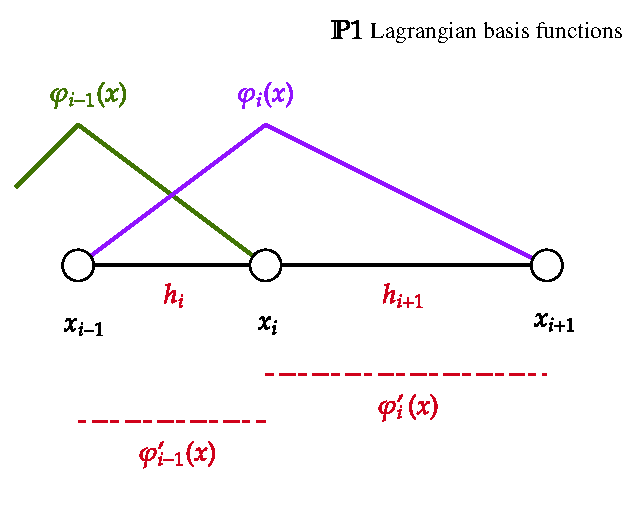
\includegraphics[width=\columnwidth]{research_project/piston/figures/p1_fem.pdf}
%     \caption{$\mathbb{P}1$ Lagrangian finite element functions.}
%     \label{fig:p1_fem}
% \end{figure}

Applying the Galerkin principle to solve PDEs, 
we enforce the orthogonality of the residual to the functional space $V_h$. 
%This is equivalent to enforcing the orthogonality to each basis function of the space, 
%so we get an algebraic system with the same number of unknowns as equations.
Because the domain changes with time, 
% even if we are solving a linear system, 
both the matrices and the vectors change for each time step,
\begin{subequations}
    \label{eq:1d_fom_linear_system_operators}
    \begin{align}
        \left[\vb{M}_{h}^{n+1}\right]_{ij}           
        &= m_{\text{BDF}} \inner{\varphi_j}{\varphi_i}^{n+1}, 
        \\
        \left[\vb{A}_{h}^{n+1}\right]_{ij}           
        &= \inner{\varepsilon \grad \varphi_j}{\grad \varphi_i}^{n+1}, 
        \\
        \left[\vb{C}_{h}^{n+1}\right]_{ij}           
        &= -\inner{c \grad \varphi_j}{\varphi_i}^{n+1}, 
        \\
        \left[\vb{N}_{h}^{n+1}\right]_{ij}           
        &= b_0 \inner{u^{*, n} \grad \varphi_j}{\varphi_i}^{n+1}, 
        \label{eq:trilinear_weak_form}
        \\
        \left[\vb{\hat{N}}_{h}^{n+1}\right]_{ij}     
        &= b_0 \left(
            \inner{g \grad \varphi_j}{\varphi_i}^{n+1} + 
            \inner{\varphi_j \grad g}{\varphi_i}^{n+1}
            \right), 
        \\
        \left[\vb{F}_{{g,h}}^{n+1}\right]_{i}        
        &= -\inner{\pdv{g}{t} + b_0 g \grad g - c \grad g}{\varphi_i}^{n+1} \nonumber
        \\
        &  -\inner{\varepsilon \grad g}{\grad \varphi_i}^{n+1},
        \label{eq:1d_fom_linear_system_operators_fg}
        \\[2mm]
        \left[\vb{F}_{\vb{\hat{u}}_h}^{n}\right]_{i} &= 
            \begin{cases}
                \inner{\hat{u}_h^{n}}{\varphi_i}^{n+1},                &\text{BDF-1},
                \\[2mm]
                2\inner{\hat{u}_h^{n}}{\varphi_i}^{n+1}
                - \frac{1}{2}\inner{\hat{u}_h^{n-1}}{\varphi_i}^{n+1}, &\text{BDF-2}.
            \end{cases}
    \end{align}
\end{subequations}
This leads to the following algebraic system:
\begin{subequations}
    \begin{align}
        \label{eq:1d_fom_weak_formulation_discrete}
        m_{\text{BDF}} \vb{M}^{n+1}_h \vb{\hat{u}}_{h}^{n+1} 
        + \dt \vb{C}^{n+1}_h \vb{\hat{u}}_{h}^{n+1} 
        + \dt \vb{A}^{n+1}_h \vb{\hat{u}}_{h}^{n+1} 
        \nonumber 
        \\[2mm] 
        + \dt \vb{\hat{N}}^{n+1}_h \vb{\hat{u}}_{h}^{n+1} 
        + \dt \left[\vb{N}^{n+1}_h\left(\vb{\hat{u}}_{h}^{*}\right)\right] \vb{\hat{u}}_{h}^{n+1} 
        \nonumber
        \\[2mm] 
        = \vb{F}_{\vb{\hat{u}}_h}^{n}
        + \dt \vb{F}_{g,h}^{n+1}, 
        \\[2mm]
        \vb{\hat{u}}_h^{0} = \vb{\hat{u}}_{h,0}.
    \end{align}
\end{subequations}
The spatial boundary conditions are encoded within the matrices and the vectors. 
The initial condition is obtain via interpolation or projection.
The assembly of the forcing term in Equation \eqref{eq:1d_fom_linear_system_operators_fg}
has to be done with the FE vector representation of the functional $f_g$ 
(which can be obtained by projection or interpolation).

Regarding the forcing due to previous time steps, $\left(\vb{F}_{\vb{\hat{u}}_h}^{n}\right)$, 
although for the FOM model we could compute the inner products at each time step, 
for the Reduced Order Model we will exploit an algebraic expression of these expressions.
It can be expressed as the product between the mass matrix and the FE representation of the previous solution(s), 
\begin{equation}
    \label{eq:1d_fom_forcing_term_time_mass_matrix}
    \vb{F}_{\vb{\hat{u}}_h}^{n}= 
    \begin{cases}
        \vb{M}_{h}^{n+1} \vb{\hat{u}}_{h}^{n},                &\text{BDF-1},
        \\[2mm]
        2\vb{M}_{h}^{n+1} \vb{\hat{u}}_{h}^{n}
        - \frac{1}{2}\vb{M}_{h}^{n+1} \vb{\hat{u}}_{h}^{n-1}, &\text{BDF-2}.
    \end{cases}
\end{equation}
We point out how the time step $\dt$ has been intentionally left out of the discrete operators definition.
There are two reasons to back this decision:
\begin{itemize}
    \item Conceptually, each discrete operator encodes a spatial model, 
    in terms of a differential operator or the presence of a forcing term.
    The time step $\dt$ shows up because we first discretized the continuous problem in time. 
    Had we gone the other way around (discretizing first in space), 
    we would have found a system of ODEs with the previously defined spatial operators. 
    \item When we leverage the system approximation reduction technique, 
    we will not want to have inside the operator the presence of the time step.
    The reduced model could use a different time step, 
    or the snapshots for different parameters could be gathered for different time step values.
\end{itemize}
% The computation of the discrete initial condition $\vb{\hat{u}}_{h,0}$ is addressed in Section~\ref{sec:1d_fom_projection_interpolation}.

If we collect terms and factor out the unknowns, we get a compact linear system to be solved at each time step to advance the solution,
\begin{subequations}
    \begin{align}
        \label{eq:1d_fom_linear_system_timestep}
        \vb{K}_h^{n+1} \vb{\hat{u}}_h^{n+1} &= \vb{b}_h^{n+1}, 
        \\
        \vb{\hat{u}}_h^{0} &= \vb{\hat{u}}_{h,0};
        \\[2mm]
        \vb{K}_h^{n+1} &= \Ah{M} + \dt \left[\Ah{A} + \Ah{C} \right. 
        \nonumber 
        \\
                        &\left. + \Ah{\hat{N}} + \Ah{N}\left(\vb{\hat{u}}_{h}^{*}\right)\right],
        \\
        \vb{b}_h^{n+1} &= \vb{F}_{\vb{\hat{u}}_h}^{n} + \dt \vb{F}_{g,h}^{n+1}.
    \end{align}
\end{subequations}

\subsubsection{Summary}
The problem has been explained within three levels of abstraction: 
continuous with strong and weak formulations, 
semi-discrete in time with the approximation of the time derivative, 
and fully discretized with the additional FEM representation of the solution.
To discretize the nonlinear term, 
the convective velocity has been extrapolated with a second order scheme.
% to obtain a sufficiently stable algebraic system.

% \mytodo{Add text: how does the semi-discretization play with the stability of the system?
% What about the convergence rates?} 

A lifting of the Dirichlet boundary conditions has been introduced, 
which leads to an additional forcing term and the homogenization of the boundary conditions.
Hence, we will focus in the solution of an homogeneous boundary value problem.
This fact will prove useful when we get into 
the implementation details of the reduction procedure.

\end{document}